%%=============================================================================
%% Use case
%%=============================================================================

\chapter{usecase}
\label{ch:usecase}

\section{Inleiding}

In dit hoofdstuk wordt er aan de hand van de verzamelde kennis en het vooropstelde model een bedrijfssituatie geanalyseerd en besproken. Het bedrijf dat onder de loep genomen wordt, is TUI. Het bedrijf is al enkele jaren bezig met de overschakeling van een monolithische architectuur naar microservices. 

Eerst bespreken we waarom het bedrijf wilt veranderen van architectuur. Elk bedrijf heeft een ander doel die ze willen verwezenlijken bij een dergelijke transformatie. Het definiëren van dit doel heeft context rond de beslissingen die genomen werden.

Vervolgens wordt het model uit hoofdstuk \ref{ch:model} toegepast en worden de verschillende aspecten van de transformatie geanalyseerd.

Daarna wordt de manier waarop het proces verloopt, beschreven. Enkele voorbeelden van microservices worden bekeken en wordt er inzicht gegeven over hoe componenten afgesplitst worden van de monoliet. 

Tenslotte is er een overzicht van de gevolgen van deze transformatie.

\subsection{Doel en verwachtingen van de transformatie}

Zoals eerder vermeld is het doel van elk bedrijf anders. In dit geval is het doel van de transformatie om het online platform van TUI te versterken en flexibeler te maken in de steeds wijzigende toerisme sector. Een bijkomend doel is om de verschillende markten (België, Duitsland, Nederland, Engeland, Zweden, Noorwegen, Finland, Denemarken, Oostenrijk, Zwitserland en Ierland) samen te brengen in één platform. TUI heeft namelijk voor elke land een apart systeem, website en database. Het is dus niet enkel een transformatie van een monolithische architectuur naar microservices, maar het is ook de bedoeling dat verschillende systemen samengevoegd worden tot één geheel. Met andere worden is het de bedoeling om meerdere monolieten te transformeren tot één geheel van microservices.  

\subsection{Toepassing van het model}

Volgens het model wordt de impact opgedeeld in vijf pijlers:

\begin{itemize}
    \item \textbf{Tijd}: Het project is begonnen in 2020 en is nog altijd bezig. De eerste mijlsteen werd afgeleverd in 2021 en de tweede mijlsteen is voorzien begin 2022. Het doel is om eind 2023 het project af te werken. Er zijn doelen opgesteld maar slechts enkele werden op tijd opgeleverd. Dit is geen uitzondering voor projecten van deze omvang en complexiteit, maar dit zorgt voor veel extra kosten die niet voorzien waren. Arbeidscontracten die niet voorzien zijn op vertragingen, kunnen heel wat roet in het eten gooien. 
    \item \textbf{Loonkost}: In 2021 waren er tussen de 500 en 1000 mensen die werkten aan de transformatie. Dit zijn ontwikkelaars, testers, \emph{product owners}, ... . Omdat de personen die mee werken aan het project afkomstig zijn uit verschillende landen, is het moeilijk om precies te weten wat de totale loonkost is. 
    \item \textbf{Infrastructuur} : Elke markt heeft zijn eigen infrastructuur. Na de transformatie zou het merendeel gebruik moet maken van de AWS services. Uiteindelijk zou dit de kosten moeten verlagen. Mits er pas overgeschakeld wordt naar het nieuwe systeem na de transformatie, is er tijdens het project een overlap. Zolang het nieuwe systeem niet klaar is, moet het huidige systeem werkend blijven. Dit zorgt voor extra kosten tijdens het project.
    \item \textbf{Personeel} : De transformatie heeft ook een hele grote impact op het personeel. Nationale teams werden internationale teams. De mix van culturen in één team is niet altijd even eenvoudig. Het uurverschil tussen de Europese landen en India zorgt voor een extra drempel. Sommige personeelsleden voelden zich niet meer thuis in deze situatie en kozen voor een nieuwe uitdaging. 
    \item \textbf{Activiteiten} : Voor de transformatie bestonden de meeste activiteiten uit onderhoudstaken voor het \emph{legacy} systeem. Het personeel dat ingezet wordt op de transformatie ontwikkelen microservices. Dit is een groot contrast met de originele activiteiten. Voor sommige personen was dit een verbetering, voor anderen minder.
    
\end{itemize}

\subsection{Verloop van de transformatie}

TUI maakt gebruik van het \emph{Strangler pattern} om hun monoliet stapsgewijs te transformeren naar microservices, zie \ref{ch:stand-van-zaken} voor meer informatie.

Een voorbeeld hiervan is het loskoppelen van de service die informatie biedt aan \emph{Online Travel Agents} van de API.

In de monoliet is deze service onderdeel van de API. Dit houdt in dat wanneer er een aanpassing nodig was specifiek voor \emph{Online Travel Agents}, het volledige deploy proces van de API uitgevoerd moest worden.

\begin{figure}[!htb]
    \centering
    \includegraphics[height=9cm]{tuiflow.png}
    \caption{Tui monoliet \label{tuiflow}}
\end{figure}

In een microservice architectuur is deze service los gekoppeld van de API. De service bestaat uit een API \emph{gateway} en verschillend lambda's. Deze service heeft ook een afzonderlijke \emph{pipeline} voor \emph{deployment}. In de monoliet werd enkel PHP gebruikt voor deze service. Voor de microservice worden er verschillende technologieën en frameworks gebruikt. Om de AWS services automatisch te creëren wordt er gebruikt gemaakt van Terraform. De lambda's zijn geschreven in nodeJS of Python. 

\begin{figure}[!htb]
    \centering
    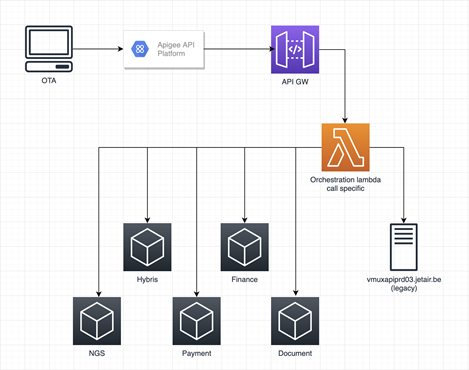
\includegraphics[height=10cm]{OTA.png}
    \caption{Tui microservice \label{tuimicro}}
\end{figure}

Een tweede voorbeeld hiervan is een \emph{micro-frontend}. De oorspronkelijke website was ontwikkeld in Drupal 7. Tijdens de transformatie werd er gekozen om de website te maken in Hybris aangevuld door React - en webcomponenten. De React componenten werden uiteindelijk opgesplitst in micro-frontends. Dit voorbeeld gaat over het prijsoverzicht die de klant te zien krijgt. Deze component is groot genoeg om zelfstandig te functioneren. 

In de oorspronkelijke website was deze module een onderdeel van de website, wat ervoor zorgde dat bij een verandering aan dit component, de volledige website \emph{gedeployed} moest worden.

\begin{figure}[!htb]
    \centering
    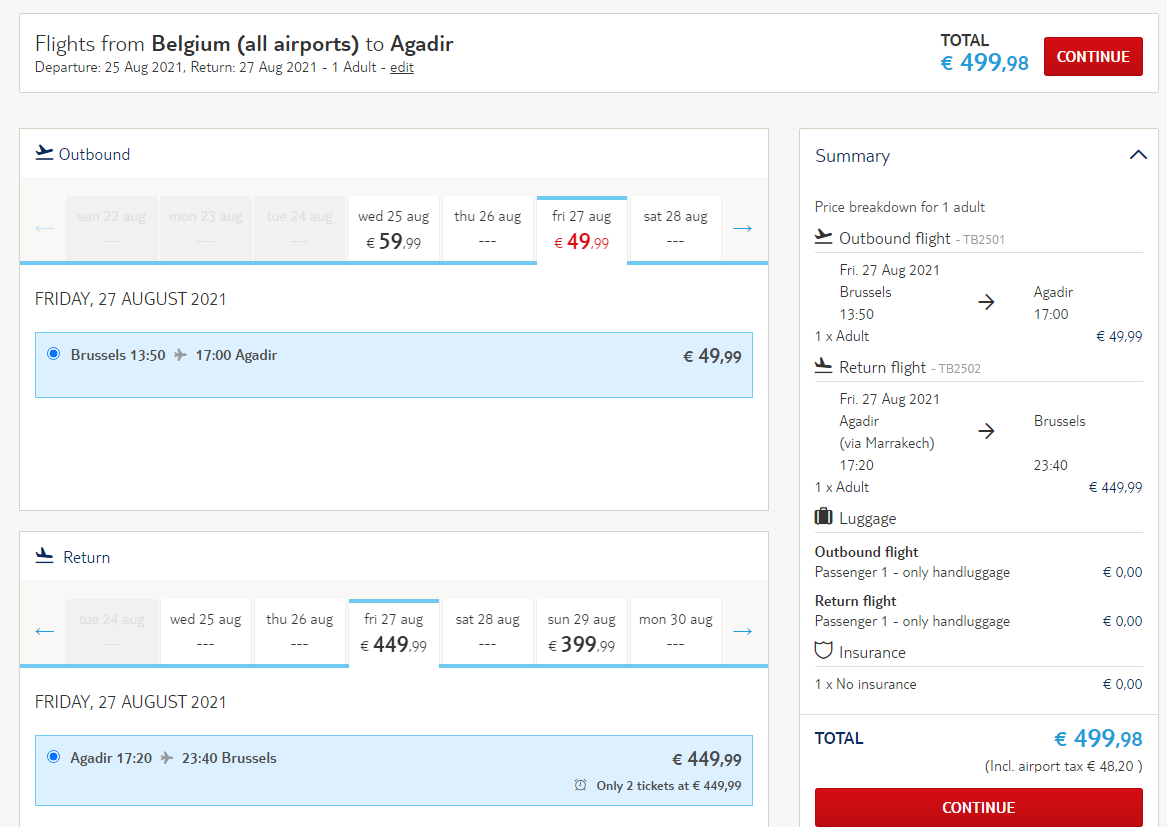
\includegraphics[height = 10cm]{priceSummary-legacy.png}
    \caption{Prijs ovezicht in de monoliet \label{pricelegacy}}
\end{figure}

Als micro-frontend is deze component losgekoppeld van de website en functioneert als een zelfstandig, geisoleerd element. Ook deze micro-frontend wordt gehost op AWS en gebruikt meerdere technologieëen. React, Javascript en Terraform.

\begin{figure}[!htb]
    \centering
    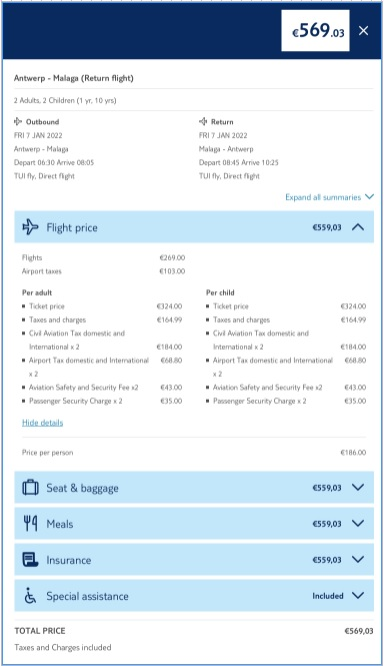
\includegraphics[height = 10cm]{PriceSummaryMicro.jpg}
    \caption{Prijs ovezicht als mircro-frontend \label{pricemicro}}
\end{figure}

\subsection{Gevolgen}

Financieel wordt er heel wat geinvesteerd in het concept van microservices en of de transformatie een succes wordt, is nog niet geweten. Deze overgang vond plaats tijdens covid-19 epidemie en de verkoop van TUI lag zo goed als stil. In theorie zou deze overgang naar microservices TUI sterker moeten maken. Het zou hun online platform een boost kunnen geven op vlak van flexbiliteit en schaalbaarheid. Voorlopig is er nog veel werk voor de boeg. Er moeten nog heel wat problemen opgelost worden en de performance moet nog verbeterd worden, zo niet zal dit project een financiële krater na laten.

In eigen land was het moeilijk om voor een bepaalde prijs het nodige personeel te vinden. Daarom werd er gekozen voor consultants van landen zoals India. Goedkope werkkrachten zorgen niet altijd voor de beste oplossingen.  

De vrijheid in keuze van technologie die microservice biedt, geven meer mogelijkheden. Dit is een stap vooruit, maar het gebruik ervan is nog niet optimaal. 

In theorie is een microservice-architectuur de beste keuze voor TUI. Maar het overgangsproces loopt niet zo vlot als verwacht en er is nog een lange weg te gaan.
